%!TEX ROOT=main.tex

\chapter{Personal development domain}\label{ch:personal-development-domain}


This section will introduce the reader to the domain of personal development.
Justification of the idea behind the application will also be presented here.

%Use empirical statements
\section{Definition of personal development}\label{sec:definition-of-personal-development}

In order to create helpful application, it is crucial to build it based on principles and ideas of personal development.
Familiarization with those will start with the definition of personal development and with Maslow's hierarchy of needs in particular.

\begin{figure}[h]
    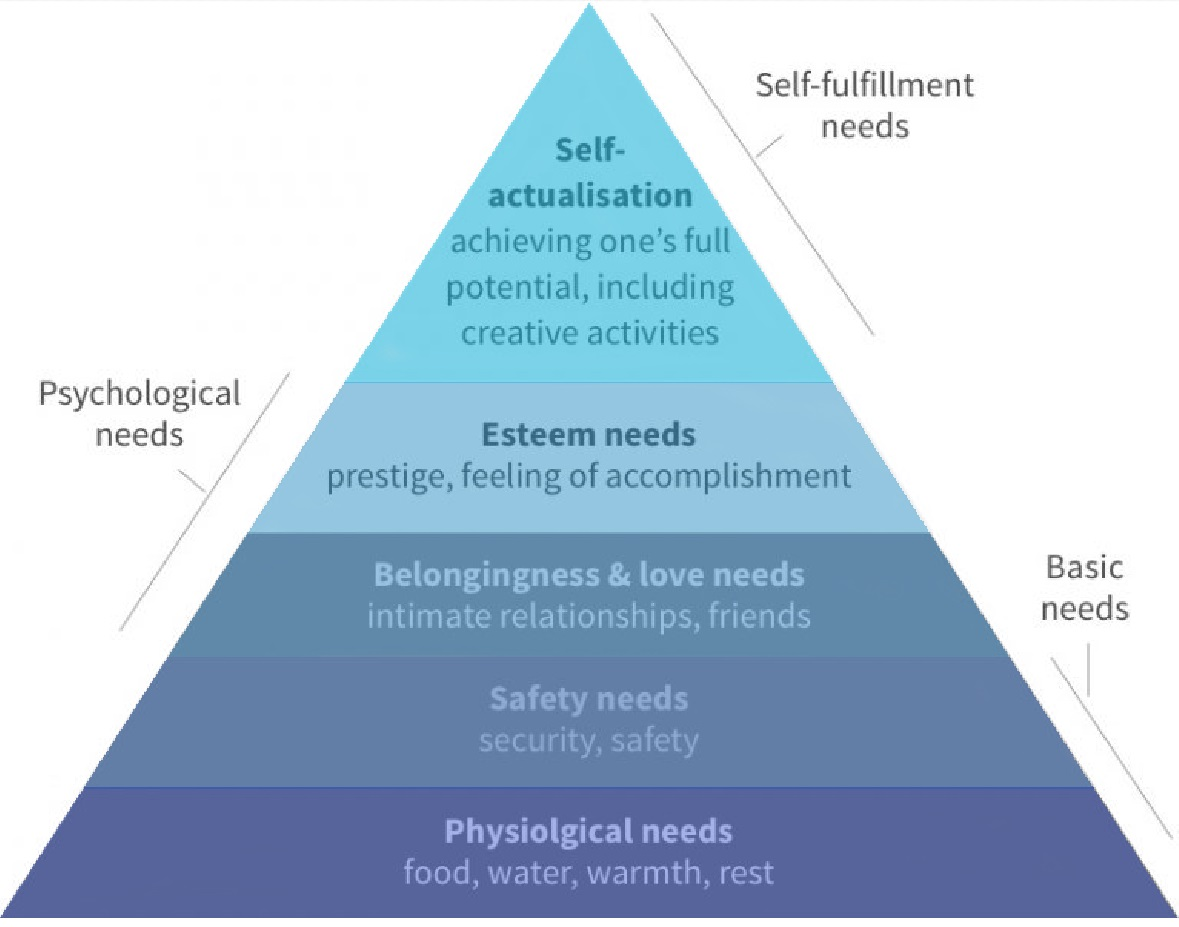
\includegraphics[width=0.75\textwidth]{images/maslows.jpg}
    \caption{Maslow's Hierarchy of Needs~\cite{maslows}}
    \label{fig:maslows}
\end{figure}




It is fair to say, that each person could give own definition of personal development.
It is nesse
It requires no special knowledge to define what personal development is.

Every person is aware of the concept of personal development.
The process of personal development is natural.
